\chapter{Design\label{cha:chapter4}}
This chapter presents the architectural design choices of the Rollup System. The Rollup System comprises Layer 1 components and Layer 2 components. The Layer 1 components encompass the Rollup smart contracts, while the Layer 2 components consist of the rollup programs and Web servers.

\section{Overview}
\todo[inline]{Put a general architecture schema}

\section{Layer 1\label{sec:designLayer1}}
Layer 1 primarily consists of the rollup smart contracts. These contracts are divided into verifier contracts and a manager contract. The verifier contracts handle rollup proof verification, while the manager contract stores the rollup state and serves as a gateway, invoking the verifiers for proof verification.

\begin{figure}[htb]
  \centering
  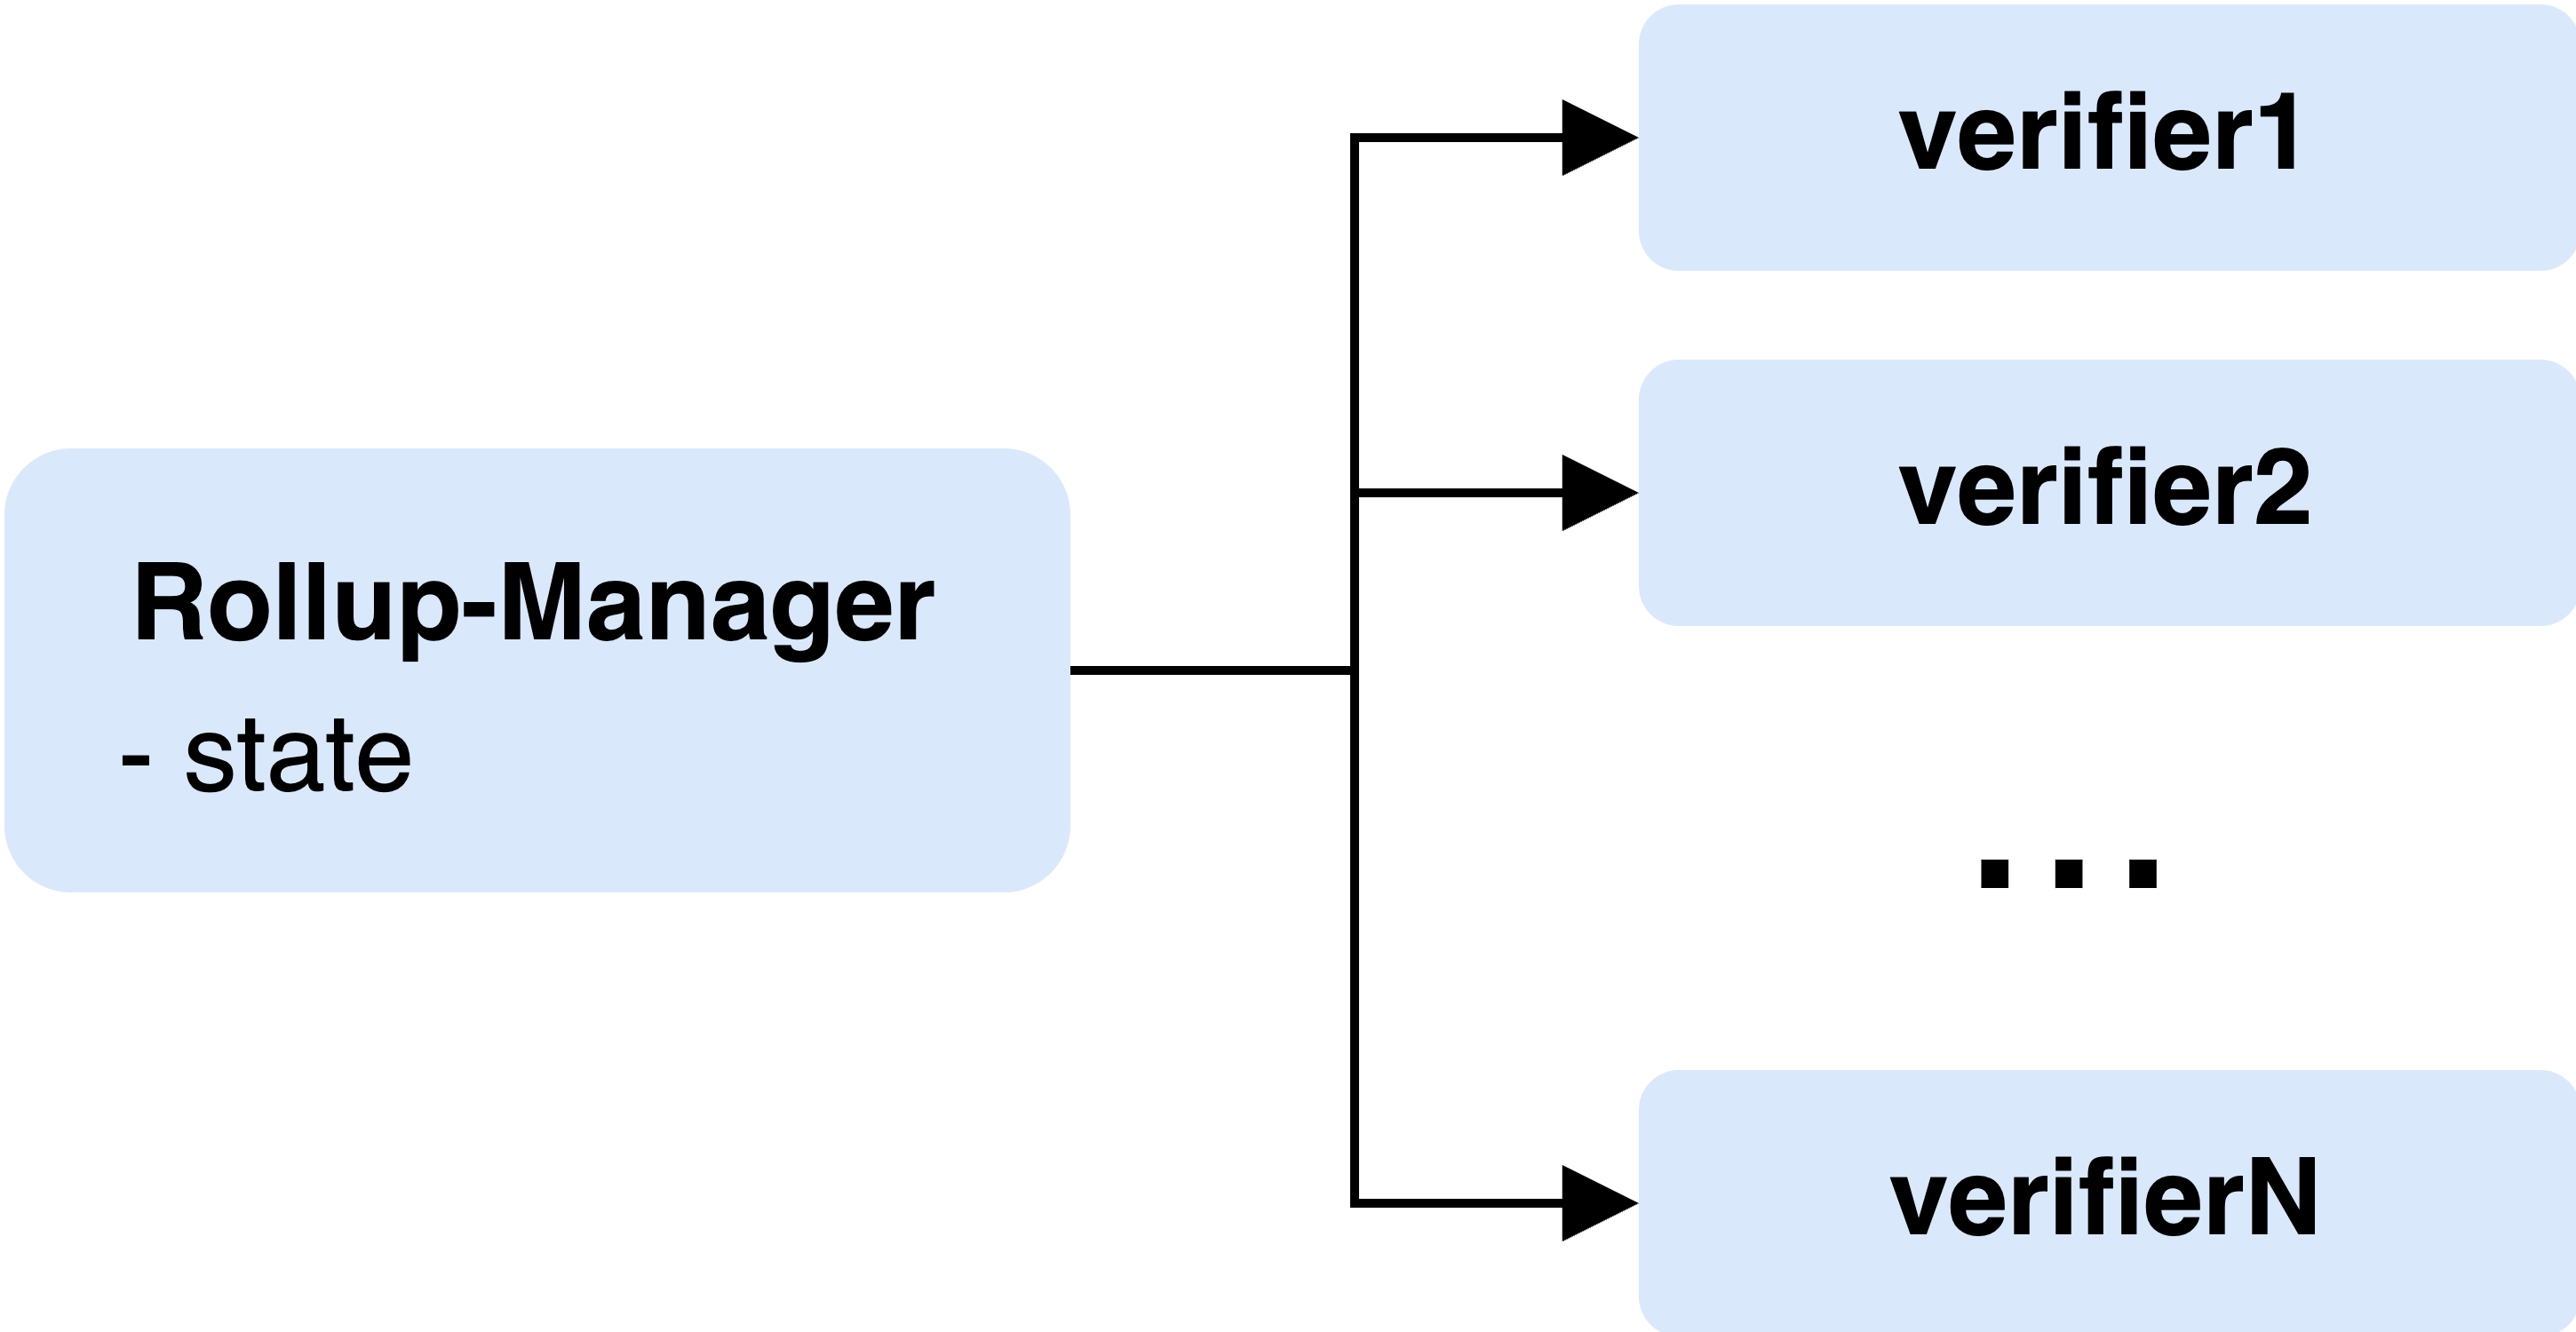
\includegraphics[width=9cm]{4_drawings-L1_general.png}
  \caption{Layer 1 Overview}
  \label{fig:Layer1overview}
\end{figure}

This modular approach enables independent upgrades of verification contracts, addressing scenarios like bugs in L2 programs. New programs may require updated verification keys, leading to deployment of corresponding verifier contracts. By having dedicated entrypoints, the rollup contract can be updated to use new verifier contracts while leaving others unaffected, necessitating only one deployment.

Another advantage of separation is reduced gas consumption: each entrypoint loads only the necessary contract code into memory. With separate contracts, the rollup contract loads only the required verifier contract for proof verification, optimizing gas usage.

\subsection{Manager Contract\label{sec:designrollupcontract}}
The Manager contract is the primary interface of the Rollup System with the blockchain. Responsible for rollup state storage and verifier contract invocation, it indirectly stores transaction history in the blockchain.

Its entrypoints handle proofs from L2 programs: forwarding proofs to relevant verifiers, verifying them, and updating storage with new state. This process is illustrated in the sequence diagram \ref{fig:Layer1sequencediagram}.

\begin{figure}[ht]
  \centering
  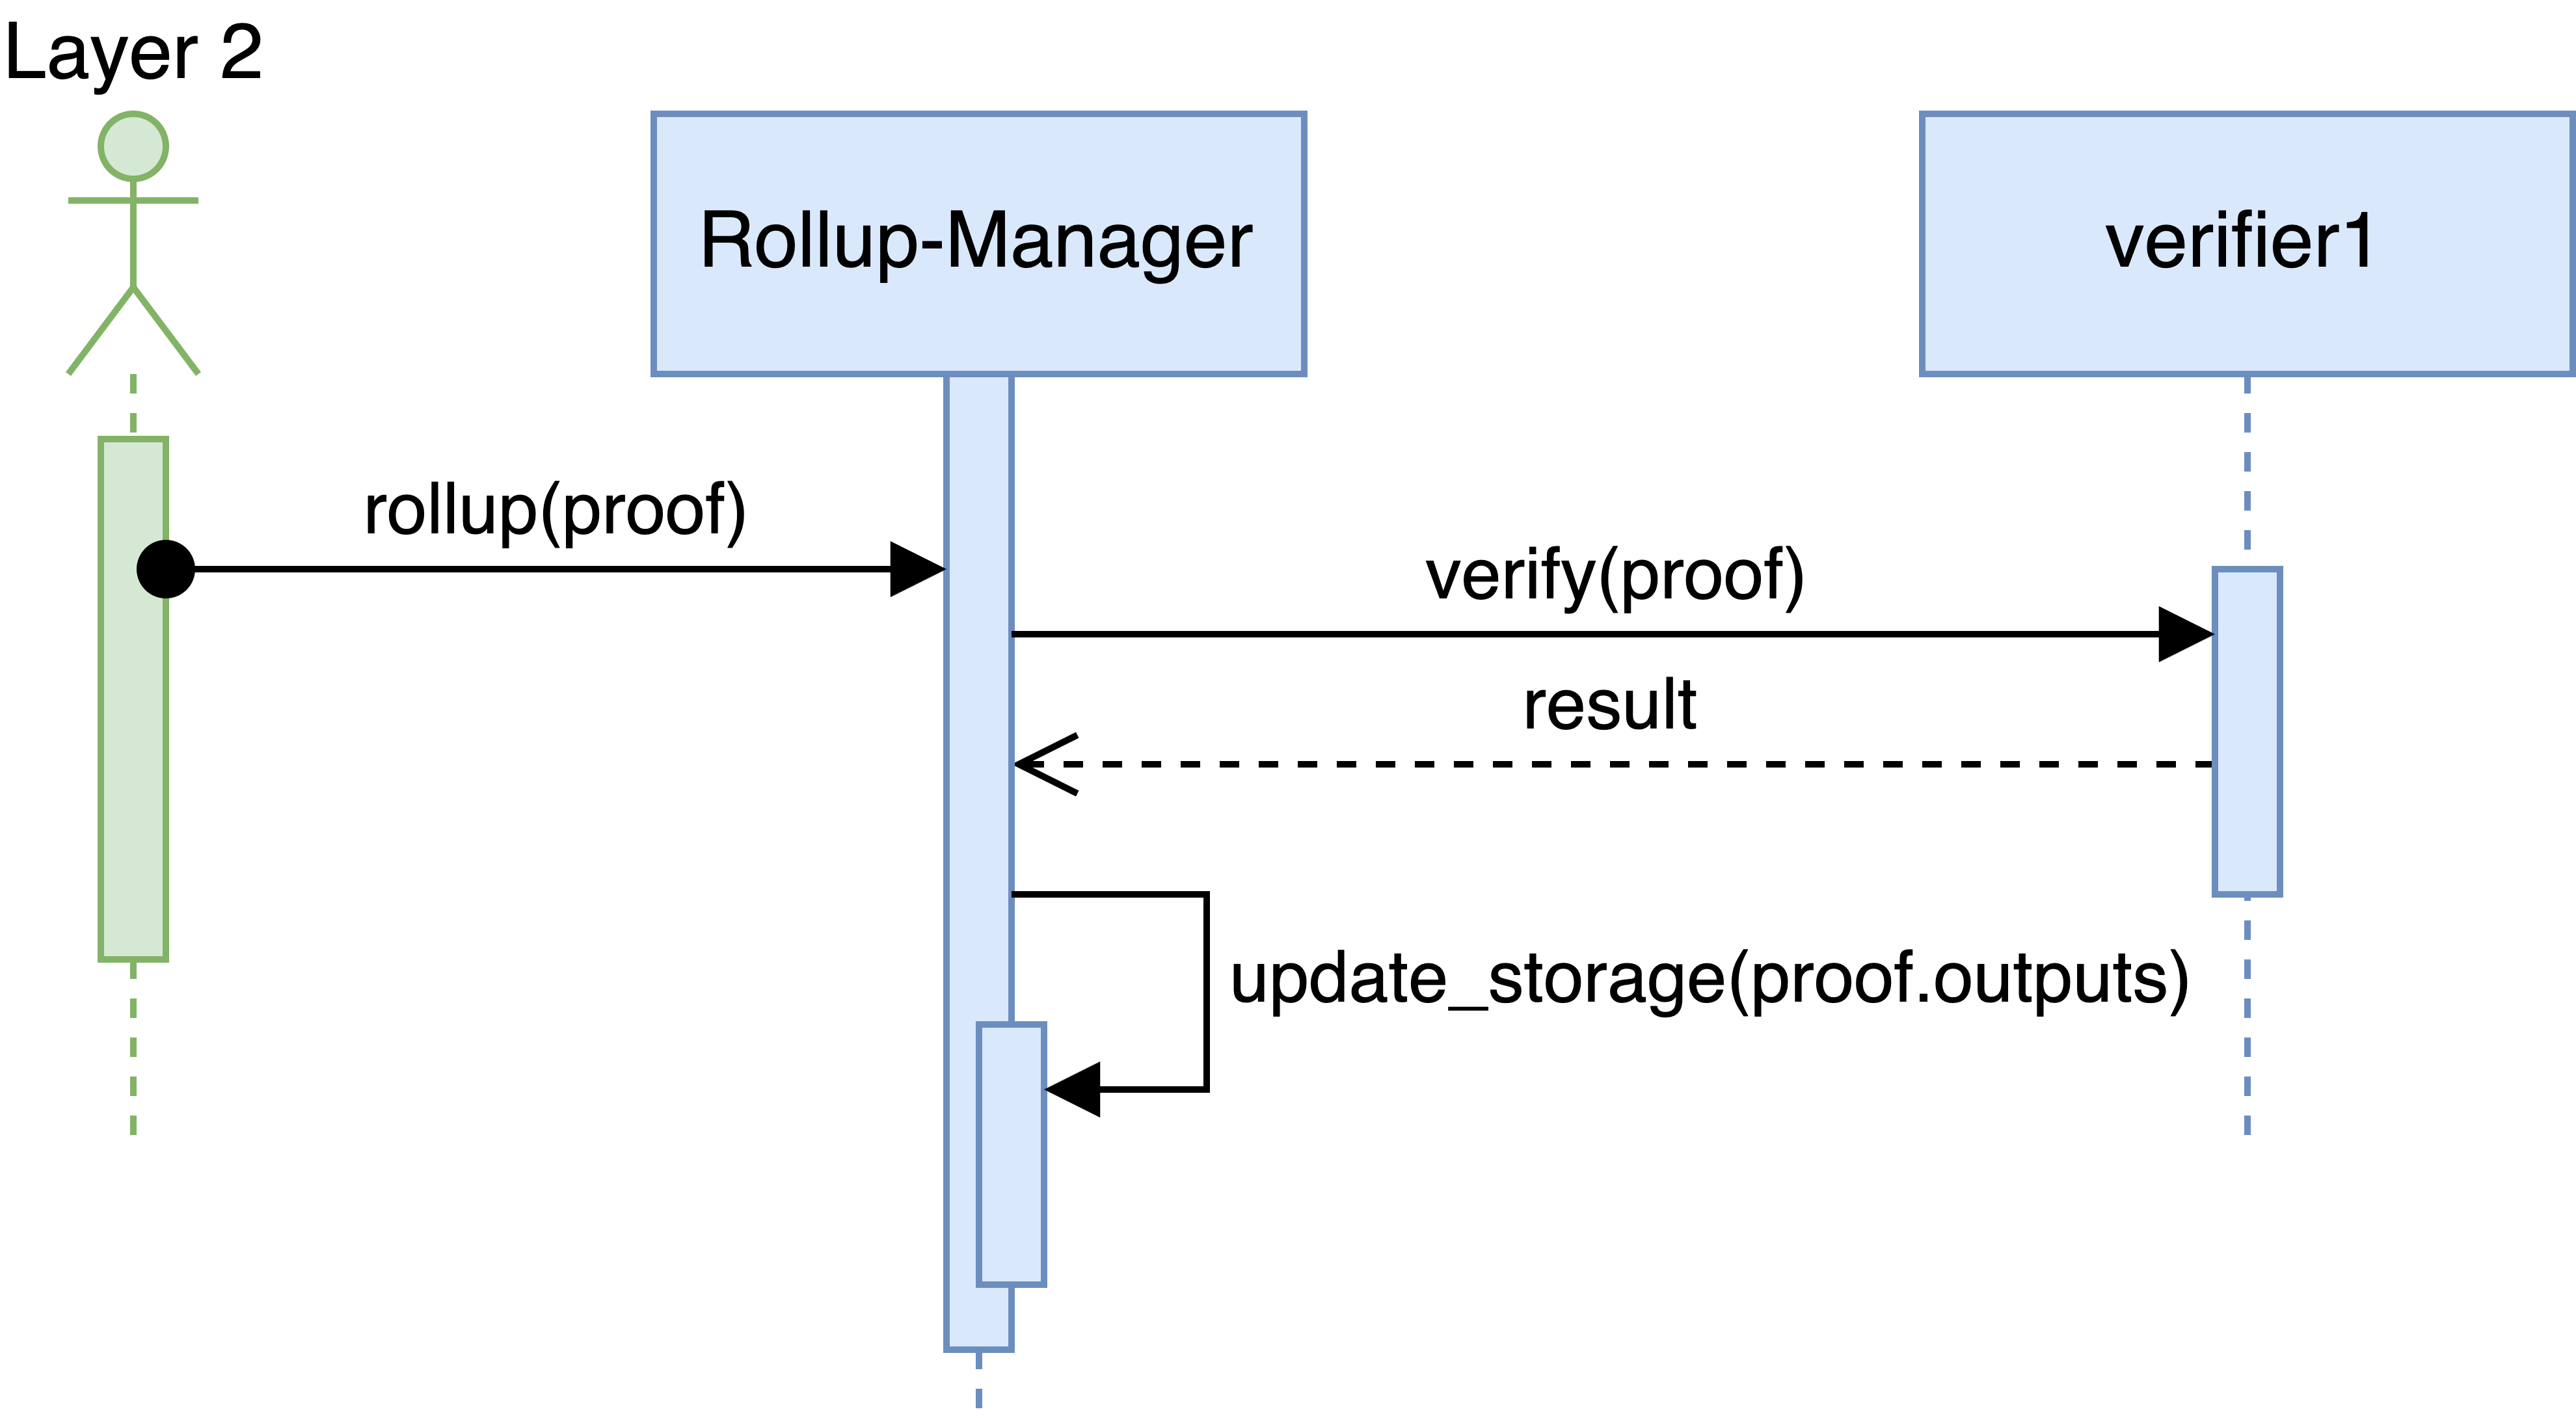
\includegraphics[width=10cm]{4_drawings-Sequence_general_L1.png}
  \caption{Layer 1 Sequence Overview}
  \label{fig:Layer1sequencediagram}
\end{figure}

\paragraph{State}
Expanding the state defined in Section \ref{sec:2_zkRollups}, the Rollup System's state includes:
\begin{itemize}
  \item \textbf{Accounts Root}: Root of the Merkle Tree containing registered accounts;
  \item \textbf{Balances Root}: Root of the Merkle Tree containing account balances;
  \item \textbf{User Map}: Map of registered users, each represented by a user index, public key, and balance.
\end{itemize}

\paragraph{Proof}
A structure with proof keys, public program inputs and program outputs. It is generated using a proving key and can be verified only using the corresponding verification key.

\paragraph{Entrypoints}
Multiple entrypoints optimize gas usage by loading only necessary code. Entrypoints for minimal functionality are:
\begin{itemize}
  \item \textbf{Register}: Register a new user;
  \item \textbf{Deregister}: Deregister a user;
  \item \textbf{Deposit}: Deposit funds;
  \item \textbf{Withdraw}: Withdraw funds;
  \item \textbf{Rollup}: Submit a rollup proof.
\end{itemize}

\subsection{Verifier Contracts\label{sec:designverifiercontracts}}
Verifier contracts validate rollup proofs. Each handles a specific proof type, and are invoked by the Rollup-Manager contract.

These contracts have no storage: they just verify proofs through an entrypoint and fail in case the verification is not successful. A challenge arises with verification key sizes: large keys can prevent deployability and execution due to gas limits, as discussed in Section \ref{subsec:gasLimit}.

\section{Layer 2\label{sec:designLayer2}}
Layer 2 consists of rollup programs and a Web Manager. Rollup programs generate zero-knowledge proofs, while the Web server exposes APIs for receiving transaction batches to be executed in a zero-knowledge context and sends proofs to the manager contract.

\begin{figure}[htb]
  \centering
  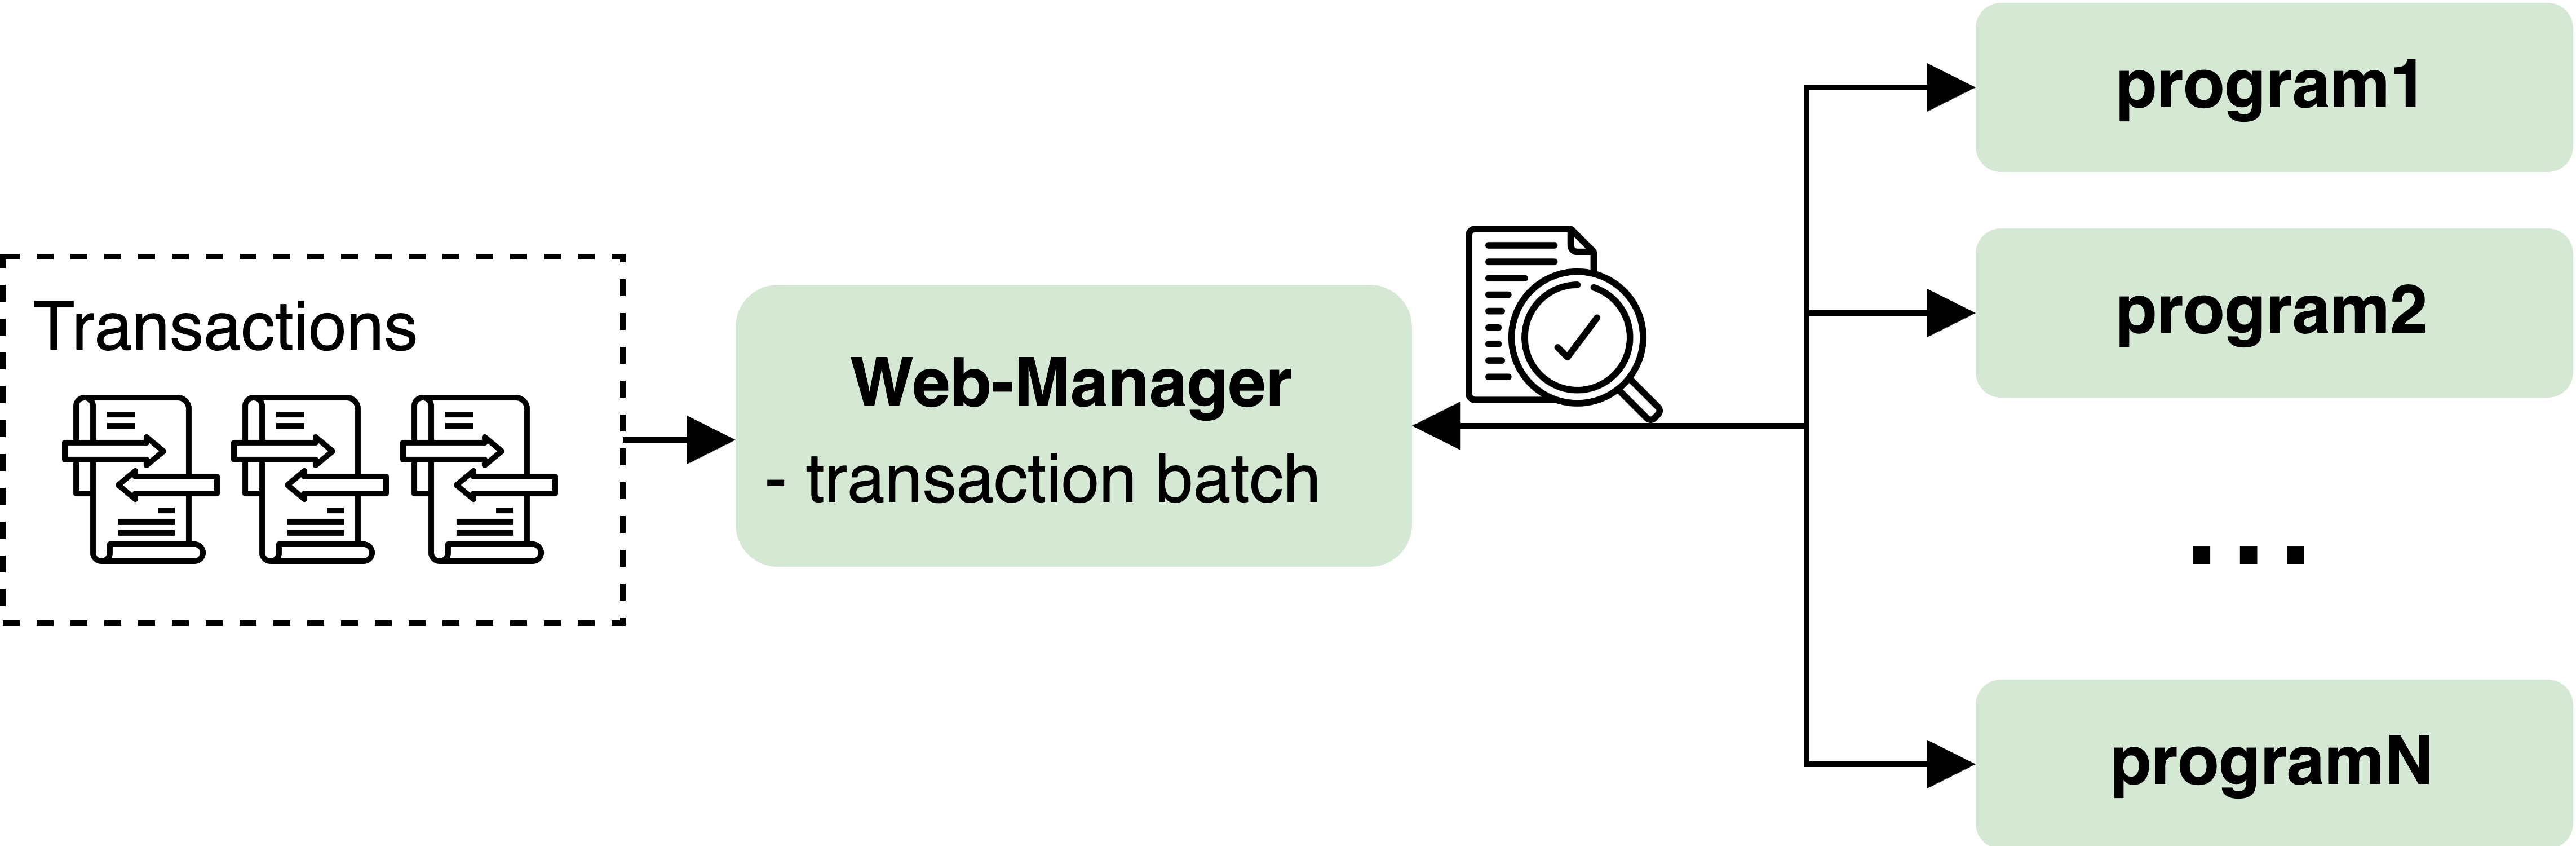
\includegraphics[width=13cm]{4_drawings-L2_general.png}
  \caption{Layer 2 Overview}
  \label{fig:Layer2overview}
\end{figure}

\subsection{Web Manager\label{sec:designwebserver}}
The Web Manager provides APIs for zero-knowledge transaction execution. It calls rollup programs and awaits their completion, sending resulting proofs to the Rollup Manager contract.

The requirement for this component is one: it must not be a bottleneck when receiving transactions and sending proofs. This can be achieved by using redundant web servers and load balancers. It should also be easily deployable and with almost no configuration needed: this can be achieved, for example, by using Docker containers.

\subsection{Rollup Programs\label{sec:designrollupprograms}}
Rollup programs are responsible for generating zero-knowledge proofs. They receive transaction batches from the Web server, execute them, and generate proofs. These proofs are sent back to the Web server, which forwards them to the manager contract. Every program has a corresponding verifier smart contract, which is able to verify the proofs generated by the program. Programs must be as small and most efficient as possible, since computing the witness for a zero knowledge proof is a very demanding operation in terms of memory and CPU usage.

Rollup programs produce as output a proof, which is a structure containing the proof keys, public program inputs and program outputs. Those elements are used by the verifier contracts to verify the proof, while the Rollup Manager contract uses program output to update the state.
